%% Overleaf			
%% Software Manual and Technical Document Template	
%% 									
%% This provides an example of a software manual created in Overleaf.

\documentclass{ol-softwaremanual}

% Packages used in this example
\usepackage{graphicx}  % for including images
\usepackage{microtype} % for typographical enhancements
\usepackage{minted}    % for code listings
\usepackage{amsmath}   % for equations and mathematics
\setminted{style=friendly,fontsize=\small}
\usepackage{hyperref}  % for hyperlinks
\usepackage[a4paper,top=4.2cm,bottom=4.2cm,left=3.5cm,right=3.5cm]{geometry} % for setting page size and margins
\usepackage{indentfirst}

\usepackage{listings,xcolor}
\lstset{
  %backgroundcolor = \color{lightgray},
  frame=l,
  language=Python,
  basicstyle=\ttfamily,
  breaklines=true,
  numberstyle=\tiny\color{gray},
  keywordstyle=\color{blue},
  commentstyle=\color{gray}\ttfamily,
  %texcl=true 
}

% Custom macros used in this example document
\newcommand{\doclink}[2]{\href{#1}{#2}\footnote{\url{#1}}}
\newcommand{\cs}[1]{\texttt{\textbackslash #1}}

% Frontmatter data; appears on title page
\title{User Manual \\Symphony}
\version{1.0}
\author{Eslab}

\setlength{\parindent}{20pt}

\begin{document}

\maketitle

\tableofcontents
\newpage

\section{Introduction}
The provided user manual is associated with a Python-based framework called \textbf{Symphony}, which is utilized for conducting radiation-based experiments. Difficulty and safety during such experiments are the most significant factors; thus, Symphony is designed to prevent human interference, using the network infrastructure and various micro-controllers, like \textbf{Raspberry Pi}, to control situations that otherwise would demand humans to interfere. 

The forenamed framework uses the \textbf{client-server} architecture to acquire the necessary features. This architecture typically uses two distinct systems, one that plays the role of the server side and the other that plays the role of the client side. Both the server and client, according to Symphony's terminology, can be referred to with a unique name. The server side can be called \textbf{Device Under Test (DUT)}, while the Client side is the \textbf{Host}. 

\section{Background}

\subsection{Radiation experiments}
Radiation experiments made in specialized facilities, where a neutron-radiation accelerator may lie, are used to evaluate the reliability of computer systems such as \textbf{FPGAs}, \textbf{CPUs}, and \textbf{ASICS} in an environment of high radiation. The most common use of the data gained from such experiments is to strengthen systems to survive in space. 

For a radiation experiment to succeed, some prerequisites are required. The most important of them is that people mustn't enter the room where charged particles are present. To accomplish this, specialized software must be made to autonomously control the systems under test inside the accelerator's room. Continuing in the current chapter, we will introduce a framework that is used to ensure both the safety of people and the integrity of the data gained in an experiment in which high radiation is present.

\subsection{Symphony}
As stated in previous chapters, Symphony constitutes a framework leveraged for conducting radiation experiments. To accomplish this, Symphony lets users customize the necessities required for an experiment. The framework provides the user with an API to instruct Symphony to handle certain crucial situations.


The Sympohy's API provides the following basic functionalities for radiation experiments:
\begin{itemize}
  \item A way to define the benchmarks to execute during the experiment
  \item A way to handle crucial situations, such as kernel panic, crashes, and more (as depicted \autoref{tab:symphony_handle}).
  \item Give the user the freedom to choose what to do in the most common situations expected in such an experiment (through some callbacks, which will be covered later). 
  \item Saves the results in easy process JSON files.
\end{itemize}

\begin{table}[h!]
\begin{center}
\begin{tabular}{ |c|c|c| } 
\hline
Situation & Handle \\
\hline
Kernel Panic & Restart \\ 
PL Crash & Restart \\  
SDCs  & LOG \\
Netowrk Error & LOG \\
System Error (recovered) & LOG \\

\hline
\end{tabular}
\caption{Crusial situations handled by Symphony}
\label{tab:symphony_handle}
\end{center}
\end{table}

\subsubsection{Architecture}
Symphony's architecture uses the Client-Server network model. As the model suggests, it uses the network infrastructure to establish a connection between two systems, one located inside the radiation room, called Device Under Test (DUT), and the other that controls the DUT device from outside, called Host. The Host is responsible for the client-side operations, while the DUT is responsible for the server side.

The architecture of Symphony can be depicted in \autoref{fig:symphony_architecture_ilustrate}. As illustrated in \autoref{fig:symphony_architecture_ilustrate}, the Host and \textbf{DUT} are connected using a gateway router. Another detail spotted in the figure is an entity called "LOGIC" and "CALLBACK" both clarified later in this sentence.  Logic constitutes hardware responsible for performing a hard reset on the DUT system. Callback, if we overuse the original terminology, it can be called a "driver". This callback instructs Symphony to perform a hard reset, when necessary, using the so-called "LOGIC" hardware in between. 

\begin{figure}[h]
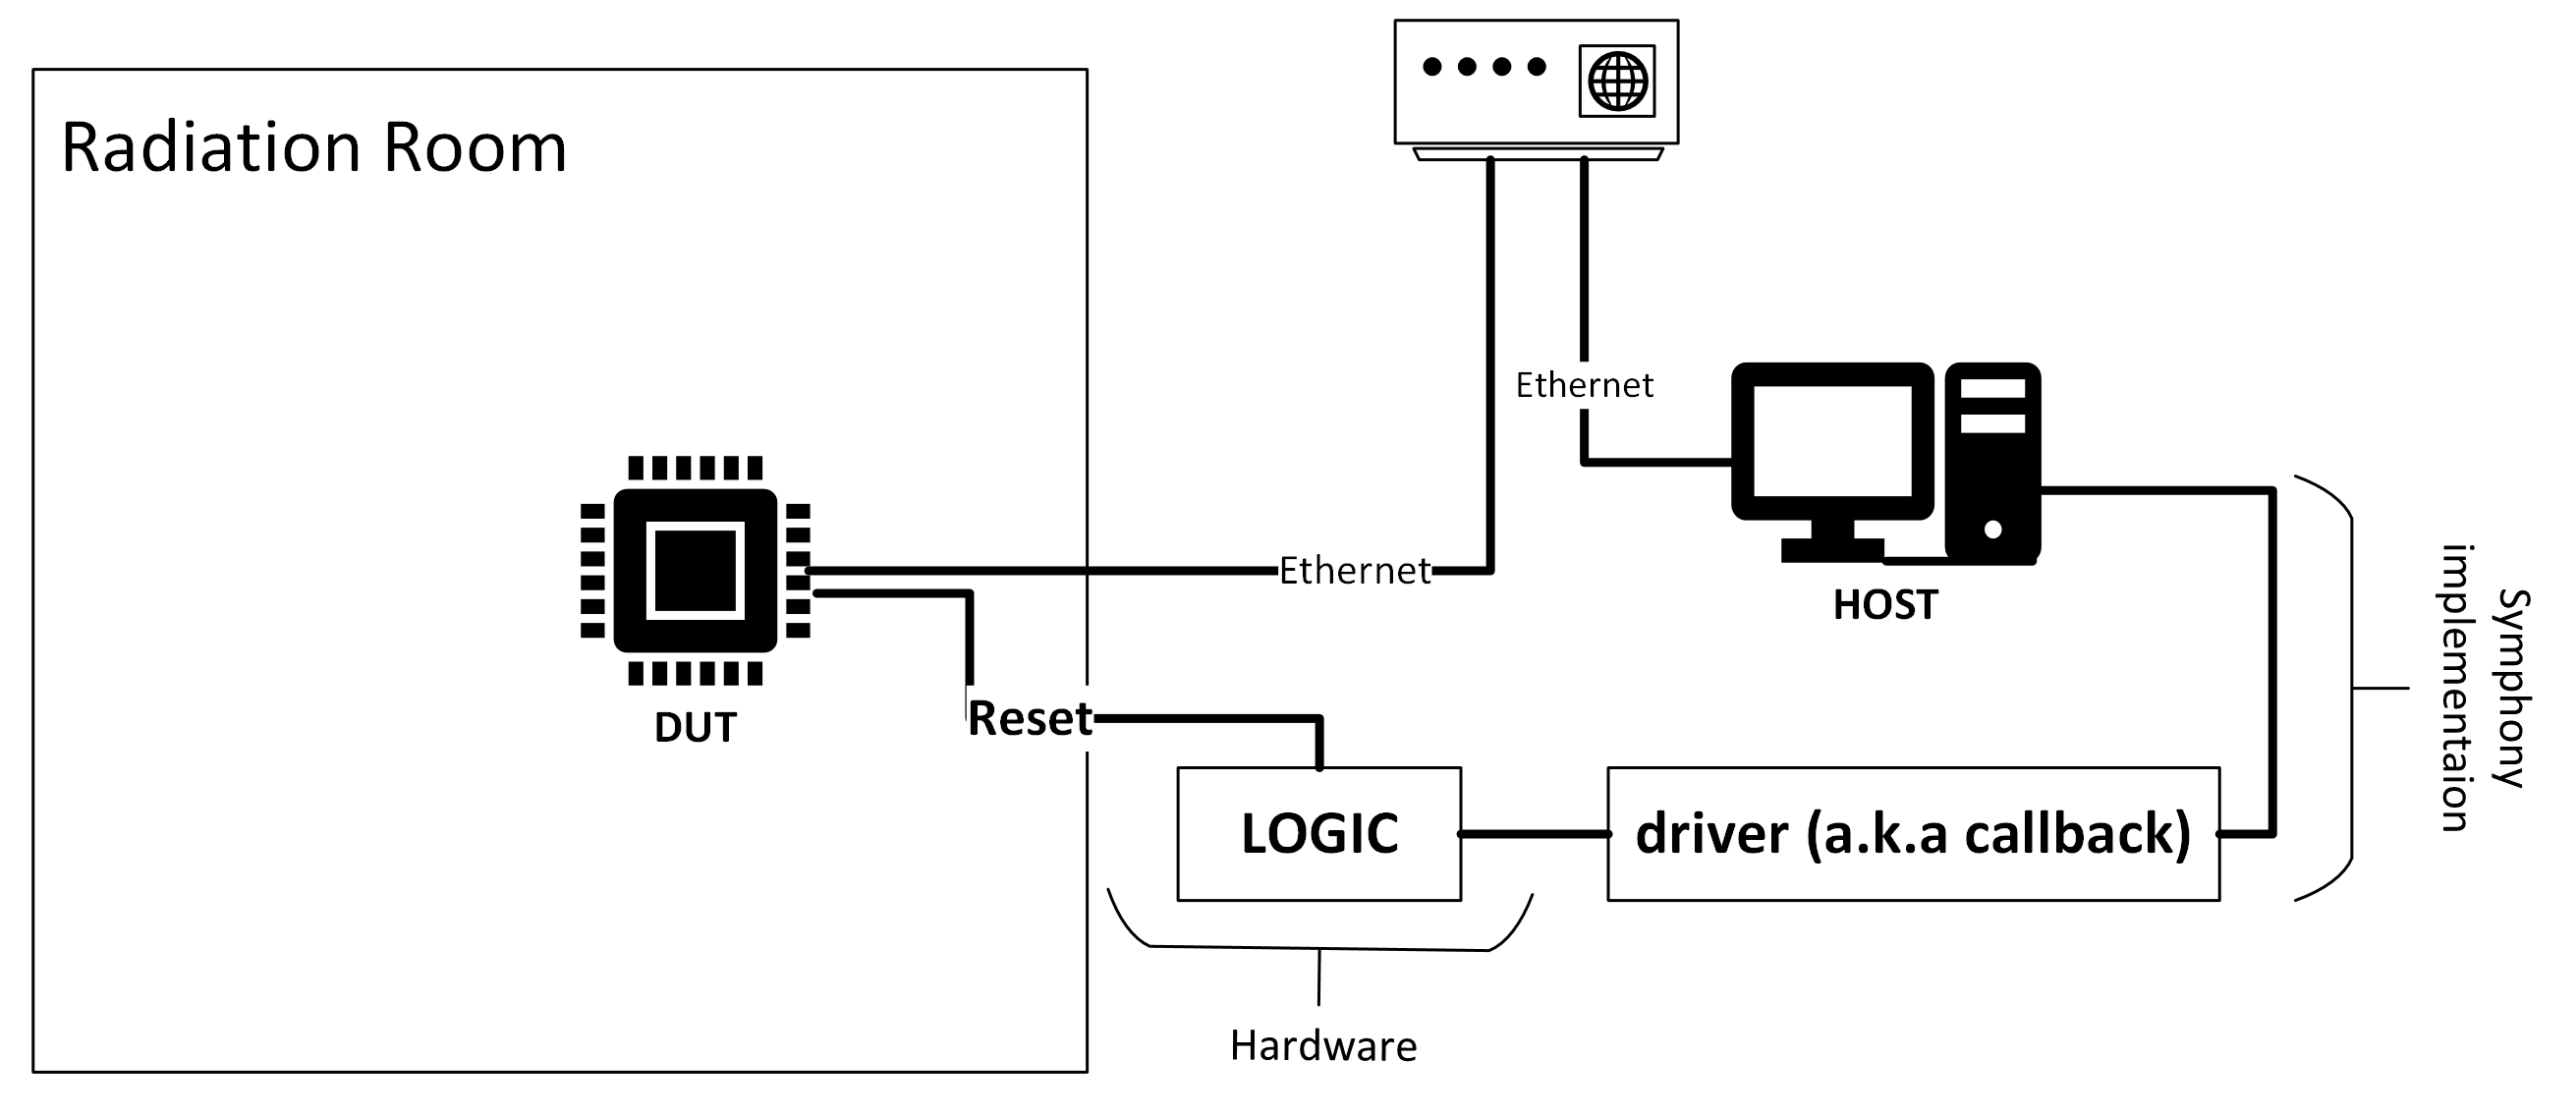
\includegraphics[width=\textwidth]{images/symphony.png}
\centering
\caption{Symphony's Architecture}
\label{fig:symphony_architecture_ilustrate}
\end{figure}

The driver (a.k.a. callback) is user-defined and varies between implementations. Section \ref{sec:user_defined_callbacks} describes how the callback is defined and how to implement such a routine.

\subsubsection{Device Under Test}
As depicted in \autoref{fig:result_message_dut}, the DUT is located inside the experiment room. This device is responsible for executing any command requested from the Host. Another task is to send back, through the network infrastructure, the results of the executed commands. The message that contains the result is in a specified dictionary format, shown in \autoref{fig:result_message_dut}.

\begin{figure}[h]
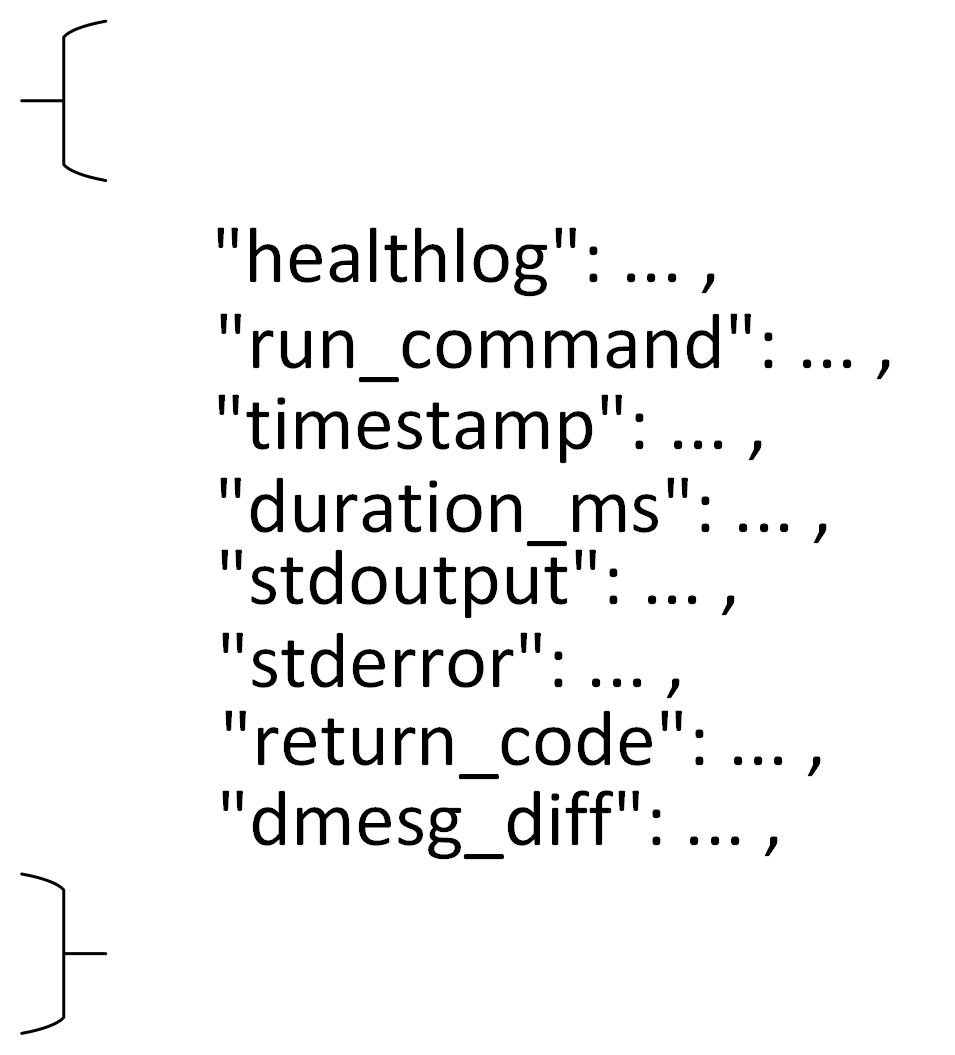
\includegraphics[width=\textwidth, height=7cm,keepaspectratio]{images/result_message_dut.png}
\centering
\caption{DUT's result message}
\label{fig:result_message_dut}
\end{figure}
\newpage

\section{Getting started}
\label{sec:getting_started}
\subsection{Requirement installation}
To install Symphony, follow these steps:
Clone the repository and navigate to the symphony directory::

\begin{lstlisting}
git clone git@github.com:unipieslab/symphony.git
cd symphony
\end{lstlisting}
Next, depending on your Linux package manager, execute the appropriate script: \\
For RedHat-based Linux, run:
\begin{lstlisting}
chmod +x install-Python<VERSION>_dnf.sh
./install-Python<VERSION>_dnf.sh
\end{lstlisting}
For Debian-based Linux, run:
\begin{lstlisting}
chmod +x install-Python<VERSION>_apt.sh
./install-Python<VERSION>_apt.sh
\end{lstlisting}
Once these steps are successfully completed, Symphony and all its dependencies will be installed. Lastly, to prepare the environment for Symphony to run, navigate to the following directory:
\begin{lstlisting}
cd host
\end{lstlisting}
Then, execute the following command:
\begin{lstlisting}
make
\end{lstlisting}
After completing this command, the host component of Symphony's client-server architecture can be started by executing the following script:
\begin{lstlisting}
./runHost.sh
\end{lstlisting}
It will then immediately attempt to connect to the DUT, if the component is up and running.

\section{Interacting with Symphony}
\subsection{JSON}
To start using \textbf{Symphony}, the user must provide certain pieces of information for the framework to start conducting the experiment. This includes a benchmark list to be executed, an experiment ID (to differentiate between results), the expected duration of the entire experiment, and other details as shown in \autoref{tab:json_entries_req}. 

The information mentioned before is defined via \textbf{JSON} format file; containing the respective fields for those listed in \autoref{tab:json_entries_req}. Not all fields listed in \autoref{tab:json_entries_req} are mandatory for Symphony's operation, some fields are used in specific scenarios, such as undervolting, while others have predefined values. The user can distinguish such fields from \autoref{tab:json_entries_req} by looking at \textbf{column 2 (Importance)}. 

Caution is required for the fields specified as "undervolted" in column 2 of \autoref{tab:json_entries_req}. Information related to undervolting can be ignored if the experiment is not undervolt-related. The respective fields in the JSON file, if not used, must remain empty, either by setting as value \textbf{"null"} or \textbf{"[]"} or \textbf{"\{\}"} depending on the type of each field.

There could be cases where the experiment requires more information than those listed in \autoref{tab:json_entries_req}. In such cases, the user can define additional fields in the JSON file to satisfy the requirements. Should the user add additional fields to the JSON file, then the respective code must be written in order to handle the extra information, see the expanding framework section.

\begin{table}[h!]
\begin{center}
\begin{tabular}{ |c|c|c| } 
\hline
JSON Entry & Importance & defaults \\
\hline
effective\_time\_per\_batch\_s & OPTIONAL & 20 \\ 
finish\_after\_total\_effective\_min & OPTIONAL & 100 \\ 
finish\_after\_total\_errors & OPTIONAL & 100 \\
voltage\_commands & UNDERVOLT & - \\
benchmark\_commands & REQUIRED & - \\
timeouts & REQUIRED & - \\ 
voltage\_list & UNDERVOLT & - \\
benchmark\_list & REQUIRED & - \\
target\_ip & REQUIRED & - \\
target\_port & REQUIRED & - \\
setup\_id & REQUIRED & - \\

\hline
\end{tabular}
\caption{Required json entries}
\label{tab:json_entries_req}
\end{center}
\end{table}
\newpage
\subsection{Interacting with the JSON}
As mentioned, the user can interact with \textbf{Symphony} via a \textbf{JSON}, by storing the desired values in the fields listed in \autoref{tab:json_entries_req}. After the filing process, the Host parses the JSON file given by the user as input and translates it into an internal dictionary, used to conduct the experiment, based on the input information. Parsing of the JSON is performed only once.

Following in this section the user will get an idea of how to use Symphony to read the corresponding JSON file of interest. 

\subsection{Load from JSON}
\subsubsection{Function signature}

\begin{lstlisting}
def load_experiment_attr_from_json_file(self, src: str)
\end{lstlisting}

\subsubsection{Description}
\begin{lstlisting}[mathescape=true, keywordstyle=\color{black}]
Read the contents of the $\textbf{JSON}$, specified in $\textbf{src}$, 
and store them in an internal dictionary. 
\end{lstlisting}

\subsubsection{Parameters}
\begin{lstlisting}[mathescape=true, keywordstyle=\color{black}]
$\textbf{src}$: The JSON file from which the entries are to be loaded
\end{lstlisting}

\subsubsection{Returns}
\begin{lstlisting}[mathescape=true, keywordstyle=\color{black}]
Nothing is returned
\end{lstlisting}

\newpage
\subsubsection{Usage Example}
\begin{lstlisting}
tester = Tester_Shell() # An instance of Symphony (Host)

json_file = "example.json" # The JSON that holds the entries
tester.load_experiment_attr_from_json_file(json_file)
\end{lstlisting}


\subsection{Load from Dictionary}
\subsubsection{Function signature}

\begin{lstlisting}
def load_experiment_attr_from_dict(self, src: dict)
\end{lstlisting}

\subsubsection{Description}
\begin{lstlisting}[mathescape=true, keywordstyle=\color{black}]
Read the contents of a $\textbf{Dicitonary}$, specified in $\textbf{src}$, 
and store them in an internal dictionary. 
\end{lstlisting}

\subsubsection{Parameters}
\begin{lstlisting}[mathescape=true, keywordstyle=\color{black}]
$\textbf{src}$: The Dictionary from which the entries are to be 
loaded
\end{lstlisting}

\subsubsection{Returns}
\begin{lstlisting}[mathescape=true, keywordstyle=\color{black}]
Nothing is returned
\end{lstlisting}

\subsubsection{Usage Example}
\begin{lstlisting}
tester = Tester_Shell() # An instance of Symphony (Host)

entries = {
    "effective_time_per_batch_s": null,
    "finish_after_total_effective_min": null,
    "finish_after_total_errors": null,
    ... # The rest of the entries
} # The dictionary that holds the entries
tester.load_experiment_attr_from_dict(entries)
\end{lstlisting}

\section{Build-in useful functions}
There are repeatedly implemented cases in a radiation-based experiment where at least one device is exposed to a source of high ionizing radiation. Such scenarios, for instance, are to monitor the devices that are being tested and to handle operations such as resetting a crashed device due to high radiation. For this reason, Symphony has implemented some built-in functions that could accelerate the development process.

Following this section, the user will learn about the available built-in functions.
\subsection{Find minimum operating voltage}
An essential part of an undervolting experiment is to find, through experimenting, a voltage value that is the minimum voltage in which the device being undervolted is operating correctly. To save time, Symphony has a built-in function that does exactly that.

\subsubsection{Function signature}

\begin{lstlisting}
def auto_undervolt_characterization(self, duration_per_bench_min: int, characterization_id: str) -> int
\end{lstlisting}

\subsubsection{Parameters}
\begin{lstlisting}[mathescape=true]
$\textbf{duration\_per\_bench\_min}$: An integer representing the number 
of minutes each benchmark should be on a specific 
(undervolted) voltage value.

$\textbf{characterization\_id}$: This field represents a string that 
corresponds to an identification for the test.

\end{lstlisting}

\subsubsection{Returns}
\begin{lstlisting}[mathescape=true]
Typically returns an integer representing the value of the 
requested voltage (aka Vmin). Otherwise, nothing is 
returned, and the user must examine the logs to determine 
Vmin.
\end{lstlisting}

\subsubsection{Usage Example}
\begin{lstlisting}
tester = Tester_Shell() # An instance of Symphony (Host)
undervolt_cmd= "Bash command for undervolting"
v_nominal = N # Where N is the initial voltage upon boot (in hexadecimal)

res = tester.auto_undervolt_characterization(n_nominal,undervolt_cmd)  # Find the Minimum operating voltage
\end{lstlisting}
(\textbf{To run the above example, there are a few preliminary steps to follow. Refer to \autoref{sec:getting_started}})
\subsection{Experiment start}
A monitoring routine that examines the behavior of a device is a complex and time-consuming procedure to develop. Such a routine must be able to retrieve integral information such as the following:
\begin{itemize}
  \item The temperature of the system.
  \item The current-voltage value (on undervolt experiments).
  \item Determine the overall health of the system
  \item Possible SDCs that occurred
\end{itemize}
Moreover, such a routine must take action in scenarios where human interference is otherwise required. One such scenario is if the device had a kernel panic and must reset to continue the experiment. 

To relieve the user from developing a routine like this, Symphony provides a built-in function that considers all the mentioned scenarios and more.

\subsubsection{Function signature}

\begin{lstlisting}
def experiment_start(self)
\end{lstlisting}

\subsubsection{Description}
\begin{lstlisting}[mathescape=true, keywordstyle=\color{black}]
Monitors the DUT system for any possible 
issues, take action when necessary, and save 
JSON formatted files that contain data from DUT (for post-
processing and analysis).

This routine, however, requires several user-implemented 
functions to perform with the expected behavior 
(see section with callbacks). 
\end{lstlisting}

\subsubsection{Parameters}
\begin{lstlisting}[mathescape=true, keywordstyle=\color{black}]
No parameters are required.
\end{lstlisting}

\subsubsection{Returns}
\begin{lstlisting}[mathescape=true, keywordstyle=\color{black}]
Nothing is returned
\end{lstlisting}


\subsubsection{Usage Example}
\begin{lstlisting}
tester = Tester_Shell() # An instance of Symphony (Host)

# User-defined functions...
# Code to make adjustments to the DUT system ... 

tester.experiment_start()

\end{lstlisting}


\subsection{Undervolt experiment}
Another routine that is often vital is a routine that performs an undervolting experiment. Such a routine must take care of a few essential actions listed below:
\begin{itemize}
  \item To reduce the voltage of the system.
  \item Evaluate the device's overall health in an (undervolted) voltage value.
  \item Execute each benchmark for the instructed total time.
\end{itemize}
Symphony has an existing implementation of such a routine, explained in the following definition.

\subsubsection{Function signature}
\begin{lstlisting}
def target_perform_undervolt_test(self)
\end{lstlisting}

\subsubsection{Description}
\begin{lstlisting}[mathescape=true, keywordstyle=\color{black}]
Performs an undervolted experiment for some
minutes, specified in the JSON. This routine makes the 
undervolting process and benchmark execution easy and 
automatic. 

This routine, however, requires several user-implemented 
functions to perform with the expected behavior 
(see section with callbacks). 
\end{lstlisting}

\subsubsection{Parameters}
\begin{lstlisting}[mathescape=true, keywordstyle=\color{black}]
No parameters are required.
\end{lstlisting}

\subsubsection{Returns}
\begin{lstlisting}[mathescape=true, keywordstyle=\color{black}]
Nothing is returned
\end{lstlisting}


\subsubsection{Usage Example}
\begin{lstlisting}
tester = Tester_Shell() # An instance of Symphony (Host)
# User-defined functions...
# Code to make adjustments to the DUT system ... 

tester.target_perform_undervolt_test()
\end{lstlisting}


\section{General purpose functions}
\subsection{power\_handler}


\subsubsection{Function signature}
\begin{lstlisting}
def power_handler(self, action: Tester_Shell_Power_Action)
\end{lstlisting}

\subsubsection{Description}
\begin{lstlisting}[mathescape=true, keywordstyle=\color{black}, showstringspaces=false]
Is responsible for shutting/resetting down the DUT system 
when necessary. The User may use this routine to 
implement custom procedures. 

Although the way each system shuts down or resets is 
almost the same, there is a variety of ways to reset 
a system in an experiment. One way is to use 
Raspberry PI's or UART modules combined with a relay to 
accomplish these two actions. Because of this variance, 
this routine requires a user-defined routine that 
explicitly instructs how the shutdown/reset procedures can 
be accomplished (See section set_callback).
\end{lstlisting}

\subsubsection{Parameters}
\begin{lstlisting}[mathescape=true, keywordstyle=\color{black}]
$\textbf{action}$: Can receive two possible actions, 
either to simulate the press of the power button 
or to simulate the press of the reset button. 
To accomplish the press of the power button, the value 
$\textbf{TARGET\_POWER\_BTN\_PRESS}$ must be passed on the routine. 
To accomplish the press of the reset button, the value 
$\textbf{TARGET\_RESET\_BTN\_PRESS}$ must be passed on the routine. 
\end{lstlisting}

\subsubsection{Returns}
\begin{lstlisting}[mathescape=true, keywordstyle=\color{black}]
Nothing is returned
\end{lstlisting}


\subsubsection{Usage Example}
\begin{lstlisting}
tester = Tester_Shell() # An instance of Symphony (Host)

tester.power_handler(Tester_Shell_Power_Action.TARGET_POWER_BTN_PRES) # Simulate the action of pressing the power button on DUT.

tester.power_handler(Tester_Shell_Power_Action.TARGET_RESET_BTN_PRESS) # Reset (reboot) the DUT system
\end{lstlisting}

\subsection{remote\_alive}

\subsubsection{Function signature}
\begin{lstlisting}
def remote_alive(self, net_timeout_s: int, ret_imediate: bool) -> bool
\end{lstlisting}

\subsubsection{Description}
\begin{lstlisting}[mathescape=true, keywordstyle=\color{black}, showstringspaces=false]
Check whether the DUT system is down. In case of any 
(communication-related) error that may encountered during 
the execution of the requested command, there will be 
attempts to finish the execution. If three attempts of 
execution have been attempted, then, the DUT
is ordered to do a hard reset.
\end{lstlisting}
\subsubsection{Parameters}
\begin{lstlisting}[mathescape=true, keywordstyle=\color{black}]

$\textbf{net\_timeout\_s}$: Represents the expected delay due to the 
network infrastructure in seconds. Users may choose their 
value of preference, but Symphony offers the built-in 
constant value $\textbf{NETWORK\_TIMEOUT\_SEC}$, which can be used 
instead.  

$\textbf{ret\_imidiate}$: Represents a logical value that allows the 
users to force the routine to return immediately after 
encountering any (communication-related) error.

\end{lstlisting}

\subsubsection{Returns}
\begin{lstlisting}[mathescape=true, keywordstyle=\color{black}]
Either $\textbf{True}$, in case the DUT is up, or 
$\textbf{False}$ in case it is down.
\end{lstlisting}


\subsubsection{Usage Example}
\begin{lstlisting}
tester = Tester_Shell() # An instance of Symphony (Host)

tester.remote_alive(Tester_Shell_Constants.NETWORK_TIMEOUT_SEC.value, False) # Check whether the DUT system is visible on the network.
\end{lstlisting}

\subsection{remote\_execute}

\subsubsection{Function signature}
\begin{lstlisting}
def remote_execute(self, cmd: str, cmd_timeout_s: int, net_timeout_s: int, dmesg_index: int, times: int, ret_imediate: bool) -> list:
\end{lstlisting}

\subsubsection{Description}
\begin{lstlisting}[mathescape=true, keywordstyle=\color{black}, showstringspaces=false]
Executes user-requested bash commands to the DUT system. 
In case of any (communication-related) error that may 
encountered during the execution of the requested command, 
there will be attempts to finish the execution. If three 
attempts of execution have been attempted, then, the DUT 
is ordered to do a hard reset. 
\end{lstlisting}

\subsubsection{Parameters}
\begin{lstlisting}[mathescape=true, keywordstyle=\color{black}]
$\textbf{cmd}$: Represents a string that is the command to execute
$\textbf{cmd\_timeout\_s}$: An integer representing the expected number 
of seconds it takes from DUT to execute the requested 
command. Timeouts like this can be estimated using the 
routine "estimate_timeouts" (see section)
$\textbf{net\_timeout\_s}$: Represents the expected delay due to the
network infrastructure in seconds. Users may choose their
value of preference, but Symphony offers the built-in
constant value $\textbf{NETWORK\_TIMEOUT\_SEC}$, which can be used
instead.

$\textbf{dmesg\_index}$: This parameter represents an integer that 
specifies the position where the last command left the 
dmesg file. The user may use this function with$\textbf { dmesg = 0}$, 
as the genuine usage of this parameter matters only in the 
internal implementation of the symphony.

$\textbf{times}$: An integer representing the number of times the DUT 
system must execute the requested command. 

$\textbf{ret\_imediate}$: Represents a logical value that allows the
users to force the routine to return immediately after
encountering any (communication-related) error.
\end{lstlisting}


\subsubsection{Returns}
\begin{lstlisting}[mathescape=true, keywordstyle=\color{black}]
Returns a list holding the results of the requested 
command. The list contains an element number equal to the 
number of times the requested command was executed. 
\end{lstlisting}


\subsubsection{Usage Example}
\begin{lstlisting}
tester = Tester_Shell() # An instance of Symphony (Host)
ls_cmd_timetout = 2 # seconds

tester.remote_execute("ls", ls_cmd_timeout, Tester_Shell_Constants. NETWORK_TIMEOUT_SEC.value, 0, 2, False)

\end{lstlisting}

\subsection{simple\_remote\_execute}

\subsubsection{Function signature}
\begin{lstlisting}
def simple_remote_execute(self, cmd: str, times: int, ret_imediate: bool) -> list
\end{lstlisting}

\subsubsection{Description}
\begin{lstlisting}[mathescape=true, keywordstyle=\color{black}, showstringspaces=false]
Is a simpler version of the corresponding remote_execute 
routine. The only difference between these two routines is 
that the simple_remote_execute routine requires fewer 
parameters than remote_execute does, making it easier to 
use in some cases where the extra parameters are 
redundant, like executing a command whose execution time 
is only a few seconds. If three attempts of execution have 
been attempted, then, the DUT is ordered to do a hard 
reset
\end{lstlisting}

\subsubsection{Parameters}
\begin{lstlisting}[mathescape=true, keywordstyle=\color{black}]
$\textbf{cmd}$: Represents a string that is the command to execute

$\textbf{times}$: An integer representing the number of times the DUT 
system must execute the requested command. 

$\textbf{ret\_imediate}$: Represents a logical value that allows the
users to force the routine to return immediately after
encountering any (communication-related) error.

\end{lstlisting}

\subsubsection{Returns}
\begin{lstlisting}[mathescape=true, keywordstyle=\color{black}]
Returns a list holding the results of the requested
command. The list contains an element number equal to the
number of times the requested command was executed
\end{lstlisting}


\subsubsection{Usage Example}
\begin{lstlisting}

tester = Tester_Shell() # An instance of Symphony (Host)
ls_cmd_timetout = 2 # seconds

tester.simple_remote_execute("ls", 2, False)

\end{lstlisting}

\subsection{set\_callback}
\label{func:set_callback}
\subsubsection{Function signature}
\begin{lstlisting}
def set_callback(self, callback_func, callback_id: Tester_Shell_Callback) -> None
\end{lstlisting}

\subsubsection{Description}
\begin{lstlisting}[mathescape=true, keywordstyle=\color{black}, showstringspaces=false]
Assigns a user-defined routine to an internal routine used 
for actions like resetting or monitoring the DUT. These 
actions can't be implemented in a way that works in every 
implementation and DUT system. Thus, the user must 
implement it for the specific scenario at hand.
\end{lstlisting}

\subsubsection{Parameters}
\begin{lstlisting}[mathescape=true, keywordstyle=\color{black}]
$\textbf{callback\_func}$: Represents a function 
pointer pointing to the user-defined function of interest.

$\textbf{callback\_id}$: Specifies which internal routine to replace 
with the user-defined routine (see section for the list of 
internal routines available for modification).
\end{lstlisting}

\subsubsection{Returns}
\begin{lstlisting}[mathescape=true, keywordstyle=\color{black}]
Nothing is returned
\end{lstlisting}


\subsubsection{Usage Example}
\begin{lstlisting}

def reset_dut():
    # Code that performs hard reset.

tester = Tester_Shell() # An instance of Symphony (Host)
ls_cmd_timetout = 2 # seconds

# How does the dut perform a hard reset?
tester.set_callback(reset_dut, Tester_Shell_Callback.TARGET_RESET_BUTTON)

# Start the experiment.
tester.experiment_start()
\end{lstlisting}

\input{general_purpose_functions/target_set_next_benchmark}
\input{general_purpose_functions/target_set_next_voltage}

\section{User defined callbacks}
\label{sec:user_defined_callbacks}



\subsection{actions\_on\_reboot}

\subsubsection{Callback signature}
\begin{lstlisting}
def __callback_actions_on_reboot(self) -> None
\end{lstlisting}

\subsubsection{Description}
\begin{lstlisting}[mathescape=true, keywordstyle=\color{black}, showstringspaces=false]
Specifies actions that must be performed 
when the DUT system reboots. For example, it can restore 
the voltage stage to where it was before rebooting. 
\end{lstlisting}

\subsubsection{Parameters}
\begin{lstlisting}[mathescape=true, keywordstyle=\color{black}]
No parameters are required.
\end{lstlisting}

\subsubsection{Returns}
\begin{lstlisting}[mathescape=true, keywordstyle=\color{black}]
Nothing is returned
\end{lstlisting}


\subsubsection{Usage Example}
\begin{lstlisting}

curr_voltage = 850 # mV

def actions_on_reboot_user_defined():
    # code ... 
    global curr_voltage
    restore_voltage(curr_voltage)

tester = Tester_Shell() # An instance of Symphony (Host)
tester.set_callback(
    actions_on_reboot_user_defined, # User defined function
    Tester_Shell_Callback.ACTIONS_ON_REBOOT # The coresponded internal callback
    )
\end{lstlisting}

\subsection{additional\_logs}

\subsubsection{Callback signature}
\begin{lstlisting}
def __callback_additional_logs(self) -> str
\end{lstlisting}

\subsubsection{Description}
\begin{lstlisting}[mathescape=true, keywordstyle=\color{black}, showstringspaces=false]
When Symphony's experiment_start method is called, except 
that it controls the DUT system, it logs important 
information about the duration of the experiment and the 
DUT system. To discourage users from modifying the 
internal logs, this callback is being used instead to 
allow the user to add additional logs if they desire. 
\end{lstlisting}

\subsubsection{Parameters}
\begin{lstlisting}[mathescape=true, keywordstyle=\color{black}]
No parameters are required.
\end{lstlisting}

\subsubsection{Returns}
\begin{lstlisting}[mathescape=true, keywordstyle=\color{black}]
A string representing the desired additional logs should 
be returned.
\end{lstlisting}

\subsubsection{Usage Example}
\begin{lstlisting}

def my_additional_logs() -> str:
    temp    = get_temp()
    voltage = get_voltage()
    return "TEMP(C):" + str(temp) + "Voltage (mV):" + str(voltage)

tester = Tester_Shell() # An instance of Symphony (Host)
tester.set_callback(my_additional_logs,


\end{lstlisting}

\subsection{detect\_cache\_upsets}

\subsubsection{Callback signature}
\begin{lstlisting}
def __callback_detect_cache_upsets(self, dmesg: str) -> None
\end{lstlisting}

\subsubsection{Description}
\begin{lstlisting}[mathescape=true, keywordstyle=\color{black}, showstringspaces=false]
Is used to specify a way to detect cache upsets that may 
be present in the DUT system.
\end{lstlisting}

\subsubsection{Parameters}
\begin{lstlisting}[mathescape=true, keywordstyle=\color{black}]
$\textbf{dmesg}:$ The current portion of DMESG contents.
\end{lstlisting}

\subsubsection{Returns}
\begin{lstlisting}[mathescape=true, keywordstyle=\color{black}]
Nothing is returned
\end{lstlisting}


\subsubsection{Usage Example}
\begin{lstlisting}

class My_tester(Tester_Shell): # Sub-class of Tester_Shell (see section 8)
    def __init__(self):
        self.total_cache_upsets = 0

    def upset_detect_user_defined(dmesg: str) -> None:
        # Analize the dmeg...
        self.total_cache_upsets += new_upsets

tester = My_tester() # An instance of Symphony (Host)
tester.set_callback(
    tester.upset_dectect_user_defined, # User-defined method
    Tester_Shell_Callback.DETECT_CACHE_UPSETS
    )

\end{lstlisting}

\subsection{is\_result\_correct}

\subsubsection{Callback signature}
\begin{lstlisting}
def __callback_is_result_correct(self, result: dict) -> bool
\end{lstlisting}

\subsubsection{Description}
\begin{lstlisting}[mathescape=true, keywordstyle=\color{black}, showstringspaces=false]
Checks whether a result is correct. Users 
may implement other mechanisms to handle a wrong result in 
addition to the check when a result is not considered 
correct.
\end{lstlisting}

\subsubsection{Parameters}
\begin{lstlisting}[mathescape=true, keywordstyle=\color{black}]
$\textbf{result}:$ The currently examined result.
\end{lstlisting}

\subsubsection{Returns}
\begin{lstlisting}[mathescape=true, keywordstyle=\color{black}]
Returns $\textbf{True}$ if the examined result is considered correct, 
otherwise $\textbf{False}$ is returned.
\end{lstlisting}

\subsubsection{Usage Example}
\begin{lstlisting}

def is_result_correct(result: dict):
    # Analize the result...
    if (correct == True):
        retrun True
    else:
        return False

tester = Tester_Shell() # An instance of Symphony (Host)

tester.set_callback(
    is_result_correct, # User-defined
    Tester_Shell_Callback.IS_RESULT_CORRECT
    )
\end{lstlisting}

\subsection{dut\_monitor}

\subsubsection{Callback signature}
\begin{lstlisting}
def __callback_dut_monitor(self, healthlog: str) -> None
\end{lstlisting}

\subsubsection{Description}
\begin{lstlisting}[mathescape=true, keywordstyle=\color{black}, showstringspaces=false]
This callback can be used to monitor the DUT system's 
resources, for example, to retrieve the temperature. Is 
possible to use this callback in combination with other 
callbacks, as depicted in the following example. 
\end{lstlisting}

\subsubsection{Parameters}
\begin{lstlisting}[mathescape=true, keywordstyle=\color{black}]
$\textbf{healthlog}:$ Constitute a string that contains crucial 
health-related information transferred from the DUT system 
(also user-defiend)
\end{lstlisting}

\subsubsection{Returns}
\begin{lstlisting}[mathescape=true, keywordstyle=\color{black}]
No parameters are required.
\end{lstlisting}

\subsubsection{Usage Example}
\begin{lstlisting}

class My_tester(Tester_Shell): # Sub-class of Tester_Shell (see section 8)
    def __init__(self):
        self.temperature = 0

    # Retrieve the temperature from DUT.    
    def monitor_dut_user_defined(self) -> None:
        # Retrieve the temperature from DUT system...
        self.temperature = dut_current_temp

    # Log the temperature of DUT.
    def my_additional_logs_user_defined(self) -> str:
        return "TEMP(C):" + str(self.temperature)

tester = My_tester() # An instance of Symphony (Host)
# Define the instructions of how to peform health-check
tester.set_callback(
    tester.monitor_dut_user_defined, # User-defined method
    Tester_Shell_Callback.DUT_MONITOR
)

# Define additional logs.
tester.set_callback(
    tester.my_additional_logs_user_defined, # User-defined method
    Tester_Shell_Callback.ADDITIONAL_LOGS.
)


\end{lstlisting}

\subsection{dut\_health\_check}

\subsubsection{Callback signature}
\begin{lstlisting}
def __callback_dut_health_check(self, tester: Tester_Shell) -> str
\end{lstlisting}

\subsubsection{Description}
\begin{lstlisting}[mathescape=true, keywordstyle=\color{black}, showstringspaces=false]
Evaluates the health of the DUT system. It is an important 
callback used in the internal implementation of Symphony 
to determine when the DUT must be reset.
\end{lstlisting}

\subsubsection{Parameters}
\begin{lstlisting}[mathescape=true, keywordstyle=\color{black}]
$\textbf{tester}:$ The instance of Symphony ($\textbf{Host}$). User may use 
every forenamed build-in function to determine the health 
of the DUT system.
\end{lstlisting}

\subsubsection{Returns}
\begin{lstlisting}[mathescape=true, keywordstyle=\color{black}]
returns an instance of the Tester_Shell_Health_Status. If 
DUT is healthy, $\textbf{Tester\_Shell\_Health\_Status.HEALTHY}$ 
must be returned, otherwhise 
$\textbf{Tester\_Shell\_Health\_Status.DAMAGED}$ must be returned.
\end{lstlisting}


\subsubsection{Usage Example}
\begin{lstlisting}

def check_health(tester: Tester_Shell):
    # Determine if the DUT is healthy.
    if (not healthy):
        return Tester_Shell_Health_Status.DAMAGED

    return Tester_Shell_Health_Status.HEALTHY

tester = Tester_Shell() # An instance of Symphony (Host)

tester.set_callback(
    check_health, # user-defined
    Tester_Shell_Callback.DUT_HEALTH_CHECK
    )
\end{lstlisting}

\subsection{request\_voltage\_value}

\subsubsection{Callback signature}
\begin{lstlisting}
def __callback_unvervolt_format(self) -> str
\end{lstlisting}

\subsubsection{Description}
\begin{lstlisting}[mathescape=true, keywordstyle=\color{black}, showstringspaces=false]
Must return the current voltage value of the regulator in 
the DUT system.
\end{lstlisting}

\subsubsection{Parameters}
\begin{lstlisting}[mathescape=true, keywordstyle=\color{black}]
No parameters are required.
\end{lstlisting}

\subsubsection{Returns}
\begin{lstlisting}[mathescape=true, keywordstyle=\color{black}]
A string representing the voltage value
\end{lstlisting}


\subsubsection{Usage Example}
\begin{lstlisting}

# For undervolting process.
current_voltage = 850 # mV

def voltage_value_user_defined() -> str
    # Code that retrives the voltage value from DUT...
    return voltage_value

tester = Tester_Shell() # An instance of Symphony (Host)
tester.set_callback(
    voltage_value_user_defined,
    Tester_Shell_Callback.REQUEST_VOLTAGE_VALUE
    )

\end{lstlisting}

\subsection{target\_power\_button}

\subsubsection{Callback signature}
\begin{lstlisting}
def __callback_target_power_button(self) -> None
\end{lstlisting}

\subsubsection{Description}
\begin{lstlisting}[mathescape=true, keywordstyle=\color{black}, showstringspaces=false]
This callback must be defined in such a way as to simulate 
the press of the power button. 
\end{lstlisting}

\subsubsection{Parameters}
\begin{lstlisting}[mathescape=true, keywordstyle=\color{black}]
No parameters are required.
\end{lstlisting}

\subsubsection{Returns}
\begin{lstlisting}[mathescape=true, keywordstyle=\color{black}]
Nothing is returned
\end{lstlisting}

\subsubsection{Usage Example}
\begin{lstlisting}

def power_button() -> None:
    # Code to simulate the press of the power button...

tester = Tester_Shell() # An instance of Symphony (Host)
tester.set_callback(
    power_button,
    Tester_Shell_Callback.TARGET_POWER_BUTTON
    )
\end{lstlisting}

\subsection{target\_reset\_button}

\subsubsection{Callback signature}
\begin{lstlisting}
def __callback_target_reset_button(self) -> None
\end{lstlisting}

\subsubsection{Description}
\begin{lstlisting}[mathescape=true, keywordstyle=\color{black}, showstringspaces=false]
This callback must be defined in such a way as to simulate 
the press of the reset button. 
\end{lstlisting}

\subsubsection{Parameters}
\begin{lstlisting}[mathescape=true, keywordstyle=\color{black}]
No parameters are required.
\end{lstlisting}

\subsubsection{Returns}
\begin{lstlisting}[mathescape=true, keywordstyle=\color{black}]
Nothing is returned
\end{lstlisting}


\subsubsection{Usage Example}
\begin{lstlisting}
def reset_button() -> None:
    # Code to simulate the press of the power button...

tester = Tester_Shell() # An instance of Symphony (Host)
tester.set_callback(
    reset_button,
    Tester_Shell_Callback.TARGET_RESET_BUTTON
    )
\end{lstlisting}

\subsection{undervolt\_format}

\subsubsection{Callback signature}
\begin{lstlisting}
def __callback_unvervolt_format(self) -> str
\end{lstlisting}

\subsubsection{Description}
\begin{lstlisting}[mathescape=true, keywordstyle=\color{black}, showstringspaces=false]
This callback is exclusively used for undervolt 
characterization, where the Symphony discovers the minimum 
voltage value in which DUT is still operating.
The task assigned for this callback is to give Symphony a 
format that can be used in each step of the undervolting 
process to reduce the voltage of the DUT system.
\end{lstlisting}

\subsubsection{Parameters}
\begin{lstlisting}[mathescape=true, keywordstyle=\color{black}]
No parameters are required.
\end{lstlisting}

\subsubsection{Returns}
\begin{lstlisting}[mathescape=true, keywordstyle=\color{black}]
A string representing the next voltage value
\end{lstlisting}

\subsubsection{Usage Example}
\begin{lstlisting}

# For undervolting process.
current_voltage = 850 # mV

def udervolt_user_defined() -> str
    global current_voltage
    disired_step = 10 # mV
    command = "apropriate command to reduce voltage" + curr_voltage
    curr_voltage = curr_voltage - disired_step 

    return command

tester = Tester_Shell() # An instance of Symphony (Host)
tester.set_callback(
    udervolt_user_defined,
    Tester_Shell_Callback.UNDERVOLT_FORMAT
    )

test.auto_undervolt_characterization(0.10, "UNDERVOLT_1")

\end{lstlisting}

\subsection{update\_all}

\subsubsection{Callback signature}
\begin{lstlisting}
def __callback_update_all(self) -> None
\end{lstlisting}

\subsubsection{Description}
\begin{lstlisting}[mathescape=true, keywordstyle=\color{black}, showstringspaces=false]
Symphony updates various variables during an experiment to 
keep track of its state. The user can use this callback to 
define their variables to update along with the 
internal variables. Variables are updated when there is a 
voltage value or a benchmark.
\end{lstlisting}

\subsubsection{Parameters}
\begin{lstlisting}[mathescape=true, keywordstyle=\color{black}]
No parameters are required.
\end{lstlisting}

\subsubsection{Returns}
\begin{lstlisting}[mathescape=true, keywordstyle=\color{black}]
No parameters are required.
\end{lstlisting}


\subsubsection{Usage Example}
\begin{lstlisting}
tester = Tester_Shell() # An instance of Symphony (Host)

tester.power_handler(Tester_Shell_Power_Action.TARGET_POWER_BTN_PRES) # Simulate the action of pressing the power button on DUT.

tester.power_handler(Tester_Shell_Power_Action.TARGET_RESET_BTN_PRESS) # Reset (reboot) the DUT system
\end{lstlisting}


\section{Expanding the framework}
Symphony is designed to create an abstraction between the user and the internal implementation. This abstraction comes at the cost of immobilizing the user from editing anything from the internal implementation. Internal functionalities may not be able to handle certain scenarios, though. For such scenarios, the user can use the inheritance model that Python delivers to expand the framework's functionalities to handle new scenarios. This chapter will describe in detail how to expand this framework.

\subsection{Inheritance Model}
Like any object-oriented programming language, Python has an inheritance model that allows the developer to create a subclass from another class. In the case of Symphony, the developer must inherit from the \textbf{Tester\_Shell} class to expand the framework's implementation. Below is an illustrative example that will clarify any issue. 


\begin{lstlisting}
class My_Tester(Tester_Shell):
    def __init__(self):
        super().__init__()
        # class Variables...
    
    def reset_button() -> None: # Method used for callback.
        # Code to simulate the press of the power button..
        
    def new_functionality_1(self):
        # Code...

    # Methods... 

tester = My_Tester() # An instance of the new implemention
tester.set_callback(
    tester.reset_button,
    Tester_Shell_Callback.TARGET_RESET_BUTTON 
)

tester.new_functionality_1()
tester.start_experiment()

\end{lstlisting}

It is important to note that the sub-class's init method must always call the \textbf{super.init()} method in order for the parent class, Tester\_Shell, to initialize its internal components. Moreover, another advantage of this implementation is that the developer can implement their callbacks inside the subclass and reference them, as shown in the previous code, to assign the corresponding callback to an internal one, using the \textbf{set\_callback} method (\autoref{func:set_callback}).

% \subsection{How to create Sections and Subsections}

Simply use the section and subsection commands, as in this example document. With Overleaf, all the formatting and numbering is handled automatically according to the template you've chosen. If you're using Rich Text mode, you can also create new section and subsections via the buttons in the editor toolbar.

\subsection{How to include Figures}

First you have to upload the image file from your computer using the upload link in the file-tree menu. Then use the includegraphics command to include it in your document. Use the figure environment and the caption command to add a number and a caption to your figure. See the code for Figure \ref{fig:frog} in this section for an example.

Note that your figure will automatically be placed in the most appropriate place for it, given the surrounding text and taking into account other figures or tables that may be close by. You can find out more about adding images to your documents in this help article on \href{https://www.overleaf.com/learn/how-to/Including_images_on_Overleaf}{including images on Overleaf}.

\begin{figure}
\centering
\includegraphics[width=0.3\textwidth]{frog.jpg}
\caption{\label{fig:frog}This frog was uploaded via the file-tree menu.}
\end{figure}

\subsection{How to add Tables}

Use the table and tabular environments for basic tables --- see Table~\ref{tab:widgets}, for example. For more information, please see this help article on \href{https://www.overleaf.com/learn/latex/tables}{tables}. 

\begin{table}
\centering
\begin{tabular}{l|r}
Item & Quantity \\\hline
Widgets & 42 \\
Gadgets & 13
\end{tabular}
\caption{\label{tab:widgets}An example table.}
\end{table}

\subsection{How to add Comments and Track Changes}

Comments can be added to your project by highlighting some text and clicking ``Add comment'' in the top right of the editor pane. To view existing comments, click on the Review menu in the toolbar above. To reply to a comment, click on the Reply button in the lower right corner of the comment. You can close the Review pane by clicking its name on the toolbar when you're done reviewing for the time being.

Track changes are available on all our \doclink{https://www.overleaf.com/user/subscription/plans}{premium plans}, and can be toggled on or off using the option at the top of the Review pane. Track changes allow you to keep track of every change made to the document, along with the person making the change. 

\subsection{How to add Lists}

You can make lists with automatic numbering \dots

\begin{enumerate}
\item Like this,
\item and like this.
\end{enumerate}
\dots or bullet points \dots
\begin{itemize}
\item Like this,
\item and like this.
\end{itemize}

\subsection{How to write Mathematics}

\LaTeX{} is great at typesetting mathematics. Let $X_1, X_2, \ldots, X_n$ be a sequence of independent and identically distributed random variables with $\text{E}[X_i] = \mu$ and $\text{Var}[X_i] = \sigma^2 < \infty$, and let
\[S_n = \frac{X_1 + X_2 + \cdots + X_n}{n}
      = \frac{1}{n}\sum_{i}^{n} X_i\]
denote their mean. Then as $n$ approaches infinity, the random variables $\sqrt{n}(S_n - \mu)$ converge in distribution to a normal $\mathcal{N}(0, \sigma^2)$.

\subsection{How to customize the template}

You may wish to customize the template for your own style, or to meet the specific needs of your documentation. If you're already familiar with LaTeX,  you can go ahead and add the packages you're familiar with to the document preamble. If you run into any problems and can't find the answers in the package documentation or in the Overleaf \doclink{https://www.overleaf.com/learn}{help library}, the forums such as \doclink{https://tex.stackexchange.com/}{TeX StackExchange} and \doclink{https://latex.org/forum/}{LaTeX Community} are a great source of answers.

Some details on how to customize a .cls file (which sets the layout and overall format of the various elements of the template) can be found at \doclink{https://www.overleaf.com/learn/latex/Writing_your_own_class}{Writing your own class}, and \doclink{http://texdoc.net/pkg/clsguide}{\LaTeX2e\ for class and package writers}. 

\end{document}
